\chapter{RESULTADOS PARCIAIS}{}
O capitulo a seguir trata dos resultados parciais obtidos durante a execução do projeto. Estes resultados são fundamentais para avaliar o progresso do trabalho e identificar áreas que necessitam de ajustes ou melhorias. A análise dos dados coletados até o momento permite uma compreensão mais profunda do fenômeno estudado e fornece \textit{insights} valiosos para as próximas etapas da projeto proposto.  

\section{Validação do Hardware}
Como forma de validar o filtro e condicionador de sinais, foram realizados testes preliminares na protoboard, a Figura \ref{fig:protoboard} apresenta o circuito preliminar desenvolvido. O objetivo desses testes foi verificar se o circuito funcional em simulação no \textit{software} multisim estava de acordo com o comportamento esperado na prática. Após a validação do hardware, foi possível observar que o filtro e o condicionador de sinais apresentaram um desempenho satisfatório, atendendo aos requisitos estabelecidos para o projeto. Desenvolvendo por fim, uma versão final do circuito em uma PCI, garantindo maior estabilidade e confiabilidade no funcionamento do sistema. Assim como apresentado na Figura \ref{fig:pcb1} e Figura \ref{fig:pcb2}.

\begin{figure}[h]
    \centering
    \caption{Teste preliminar do circuito em protoboard.} 
    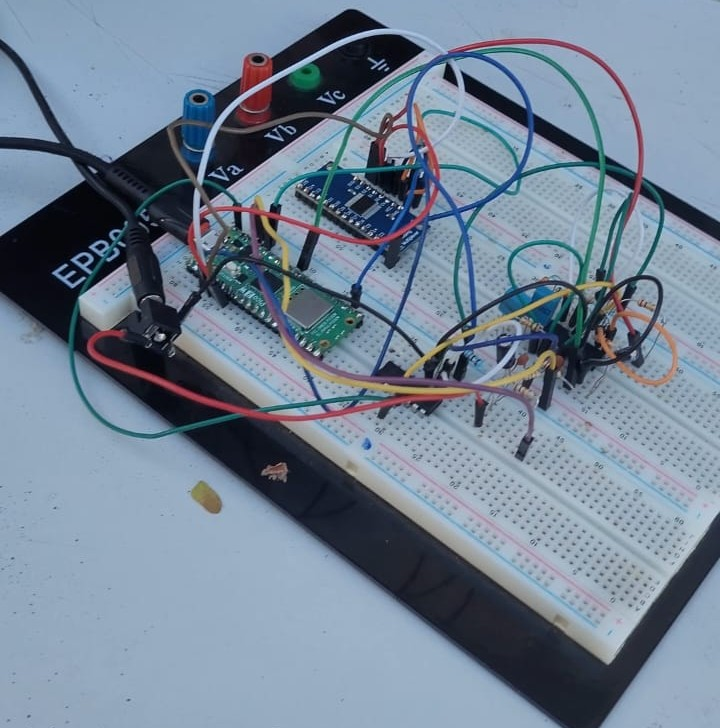
\includegraphics[width=0.7\textwidth]{figuras/circuito_proto.jpeg}
    \label{fig:protoboard}\\
    \autoria{Autoria Própria.}
\end{figure}


Concluída a etapa de validação do \textit{hardware}, foram realizadas duas campanhas de
coleta de dados com o sistema embarcado já em operação normal. A
primeira teve como objetivo aferir a precisão das leituras de corrente
do sistema frente a um instrumento de referência e ao valor nominal
informado pelo fabricante do motor utilizado nos testes. A segunda
buscou avaliar o comportamento do sistema diante de uma condição de
falha real na alimentação elétrica, especificamente a perda de uma das
fases durante a operação do motor. Ambos os ensaios utilizaram o mesmo
motor de indução trifásico, modelo WEG W22, presente no laboratório de máquinas elétricas no Centro Multidisciplinar da Universidade
Federal do Oeste da Bahia (UFOB), em Bom Jesus da Lapa.

\section{Validação da Medição de Corrente}


Para verificar a exatidão das leituras de corrente fornecidas pelo
sistema, o motor WEG W22 Figura~\ref{fig:motor_w22} foi energizado em
regime nominal e monitorado simultaneamente pelo sistema embarcado e
por um alicate amperímetro Minipa ET-3810C
Figura~\ref{fig:alicate_minipa}, instrumento com função \textit{True
RMS} utilizado como referência de comparação.

\begin{figure}[htb]
    \centering
    \caption{Motor de indução trifásico WEG W22 utilizado nos ensaios.}
    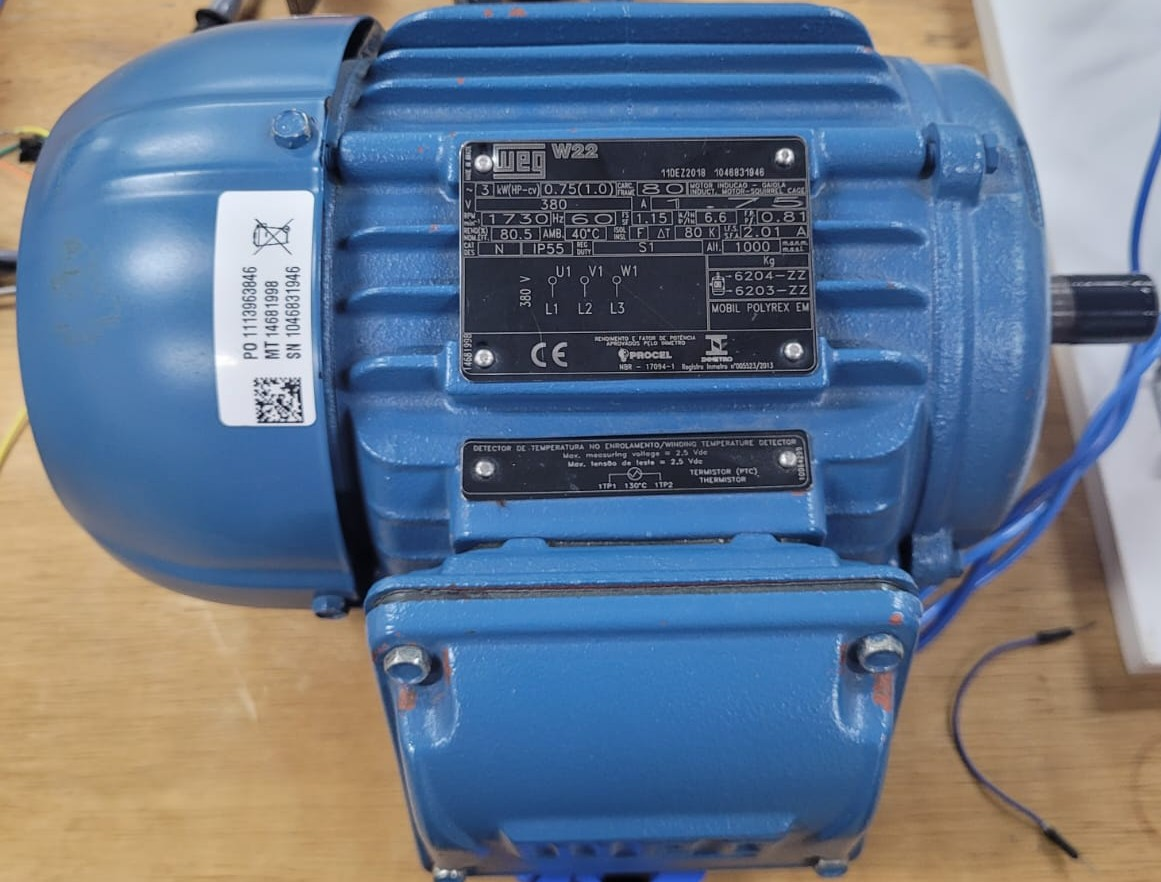
\includegraphics[width=0.5\textwidth]{figuras/motor.jpeg}
    \label{fig:motor_w22}\\
    \autoria{ Autoria Própria.}
\end{figure}

\begin{figure}[htb]
    \centering
    \caption{Alicate amperímetro Minipa ET-3810C utilizado como referência de medição.}
    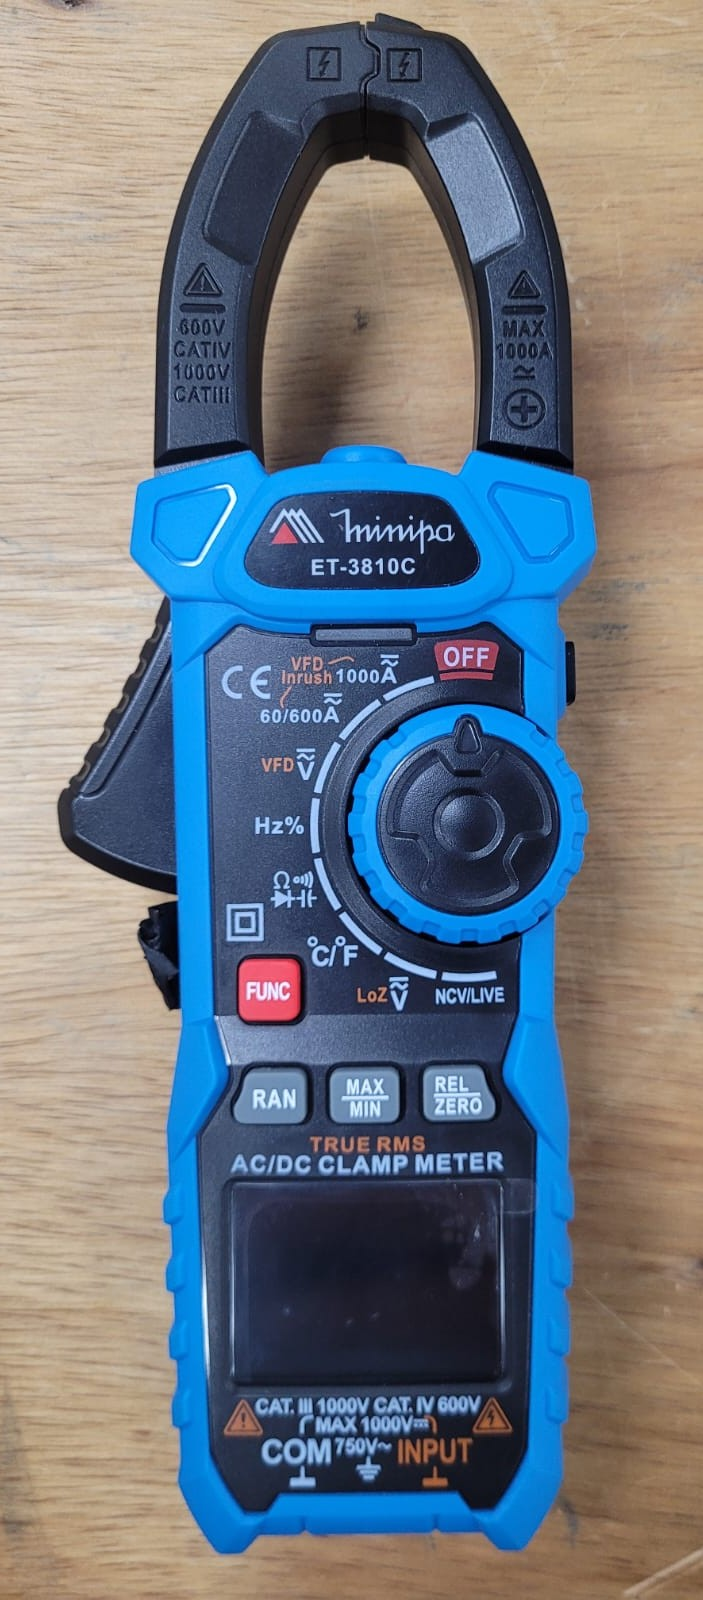
\includegraphics[width=0.4\textwidth]{figuras/Alicate.jpeg}
    \label{fig:alicate_minipa}\\
    \autoria{ Autoria Própria.}
\end{figure}

De acordo com a placa de identificação do motor, a corrente nominal em
380 V é de 1,15 A. Nas mesmas condições de operação, o alicate Minipa
indicou uma leitura de 1,15 A, enquanto o sistema embarcado registrou
uma corrente próxima de 1,1 A, valor que se manteve estável ao longo
das amostras coletadas. Essa diferença corresponde a um erro relativo
de aproximadamente 4,3\% frente ao instrumento de referência, o que é
compatível com a faixa de erro típica de sensores de corrente não
invasivos do tipo SCT-013 sem compensação adicional de ganho
(Quadro~\ref{quadro:comparacao_corrente}).

\begin{quadro}[htb]
    \centering
    \caption{Comparação entre a corrente nominal, a medição de referência e a leitura do sistema embarcado.}
    \begin{tabular}{|l|c|}
        \hline
        \textbf{Grandeza} & \textbf{Valor} \\
        \hline
        Corrente nominal (placa do motor) & 1,15 A \\
        \hline
        Corrente medida (alicate Minipa ET-3810C) & 1,15 A \\
        \hline
        Corrente medida (sistema embarcado) & $\approx$ 1,10 A \\
        \hline
        Erro relativo (sistema x referência) & $\approx$ 4,3\% \\
        \hline
    \end{tabular}
    \label{quadro:comparacao_corrente}\\
    \autoria{ Autoria Própria.}
\end{quadro}

Esse resultado indica que, embora o sistema ainda apresente um
pequeno desvio em relação à referência, a ordem de grandeza da medição
está correta e o erro observado é aceitável para um estágio inicial de
validação, podendo ser reduzido em etapas futuras por meio de ajuste
fino do ganho de calibração de cada canal de corrente.

\section{Ensaio de Falta de Fase}


Com o objetivo de avaliar o comportamento do sistema em uma condição
real de distúrbio na rede, o mesmo motor WEG W22 foi acoplado à
bancada de testes de partida de motores do laboratório
Figura~\ref{fig:bancada_testes}.Essa bancada permitiu induzir, de forma controlada, uma condição de
falta de fase durante a operação do motor, interrompendo a alimentação
de uma das três fases enquanto as demais permaneciam energizadas.

\begin{figure}[htb]
    \centering
    \caption{Bancada de testes de partida de motores utilizada no ensaio de falta de fase.}
    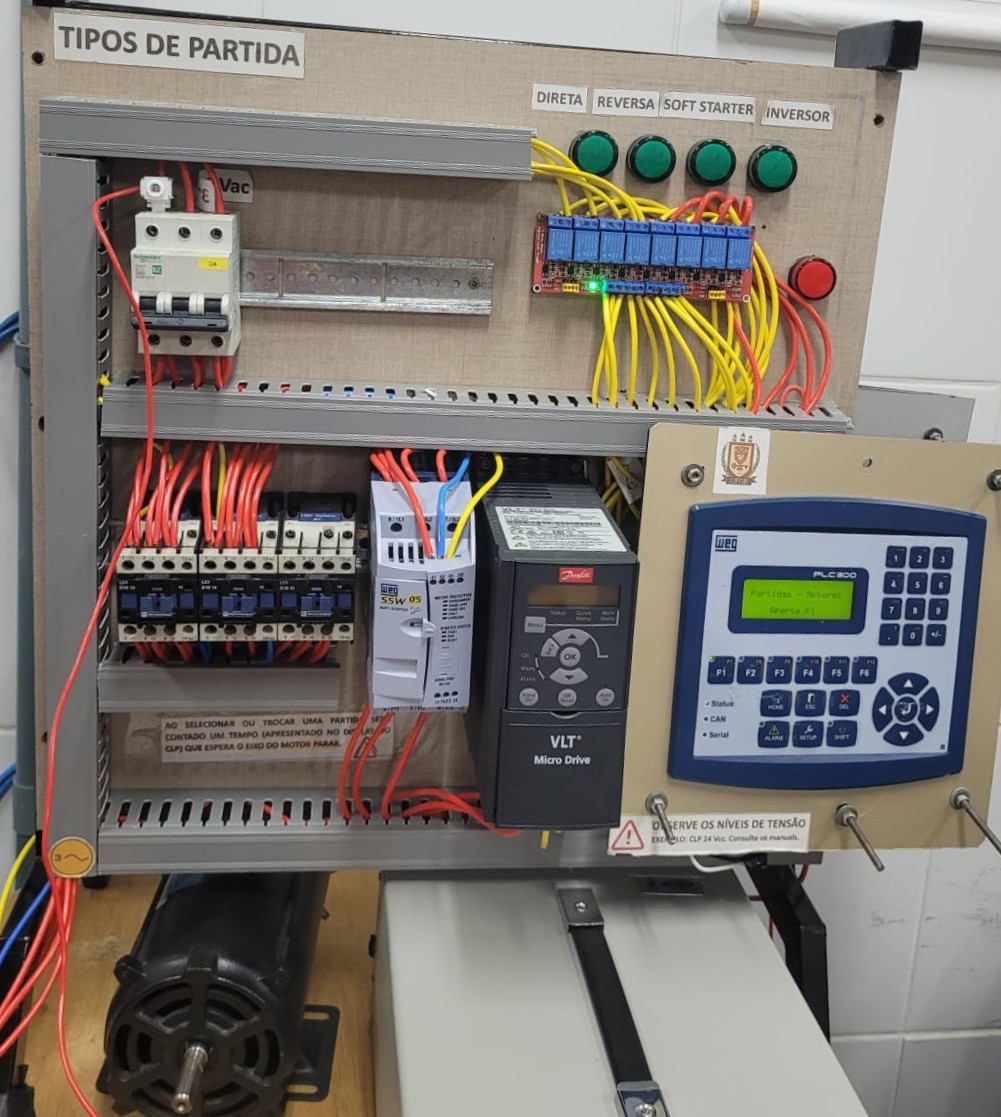
\includegraphics[width=0.6\textwidth]{figuras/bancada.jpeg}
    \label{fig:bancada_testes}\\
    \autoria{ Autoria Própria.}
\end{figure}

Durante o ensaio, o sistema embarcado manteve o registro contínuo das
correntes das três fases (L1, L2 e L3) e da tensão de rede, permitindo
observar a transição entre o regime normal de operação e a condição de
falta. As Figuras~\ref{fig:corrente_l1}, \ref{fig:corrente_l2} e
\ref{fig:corrente_l3} apresentam, respectivamente, as correntes
medidas nas fases L1, L2 e L3 ao longo do ensaio, enquanto a
Figura~\ref{fig:tensao_rede} apresenta a tensão de rede registrada no
mesmo intervalo.

\begin{figure}[htb]
    \centering
    \caption{Corrente na fase L1 durante o ensaio de falta de fase.}
    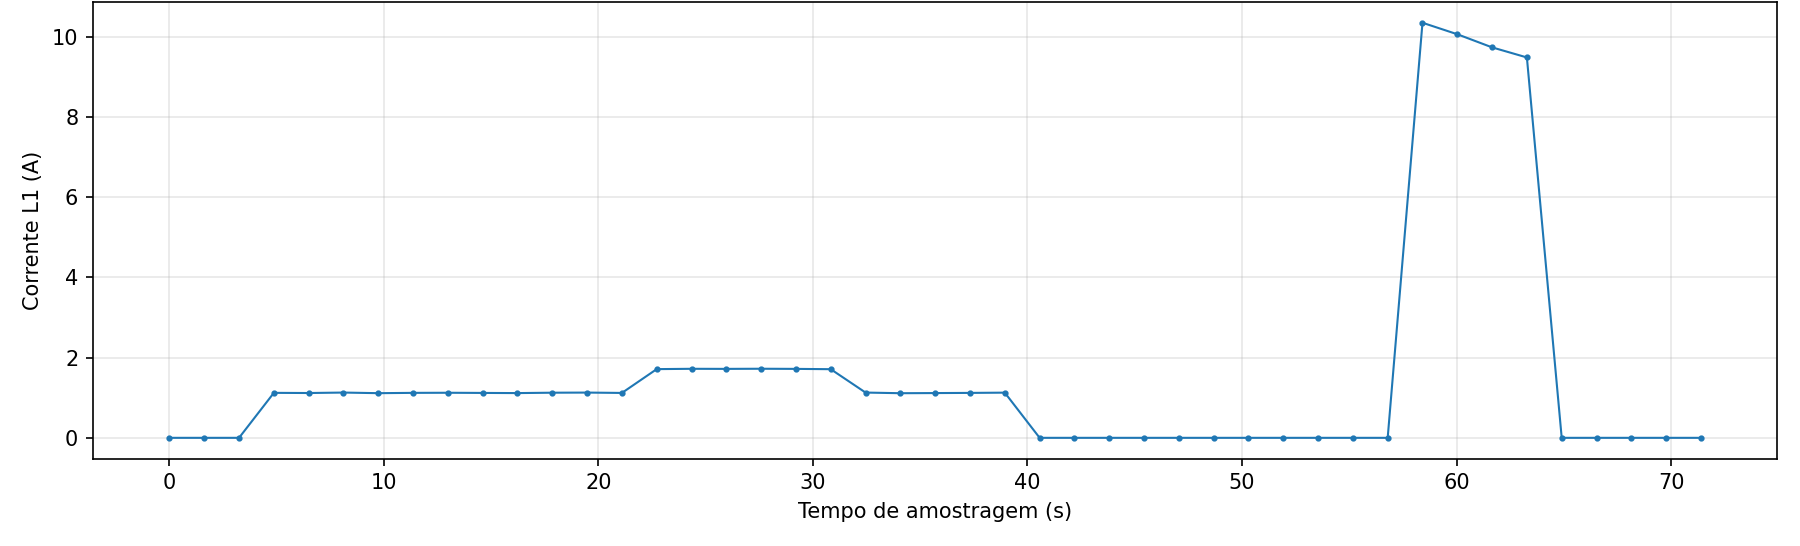
\includegraphics[width=0.85\textwidth]{figuras/I_L1.png}
    \label{fig:corrente_l1}\\
    \autoria{ Autoria Própria.}
\end{figure}

\begin{figure}[htb]
    \centering
    \caption{Corrente na fase L2 durante o ensaio de falta de fase.}
    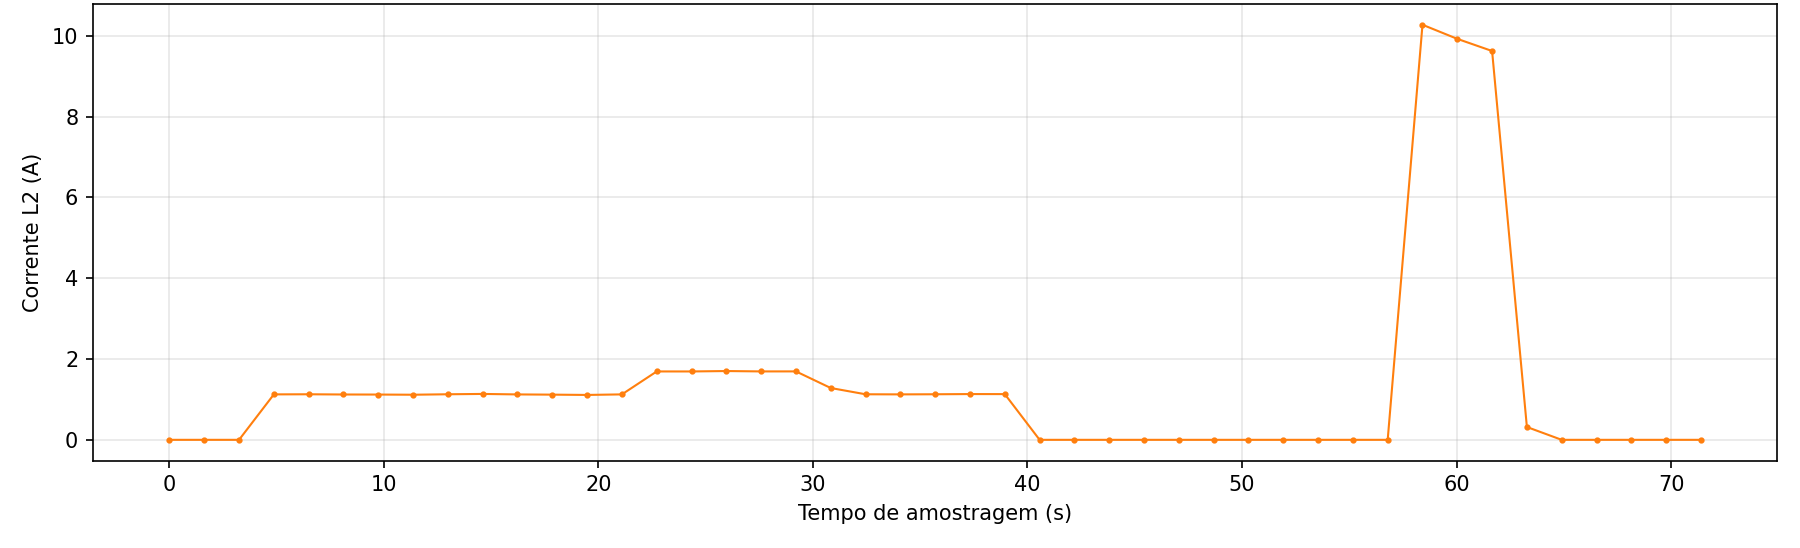
\includegraphics[width=0.85\textwidth]{figuras/I_L2.png}
    \label{fig:corrente_l2}\\
    \autoria{ Autoria Própria.}
\end{figure}

\begin{figure}[htb]
    \centering
    \caption{Corrente na fase L3 durante o ensaio de falta de fase.}
    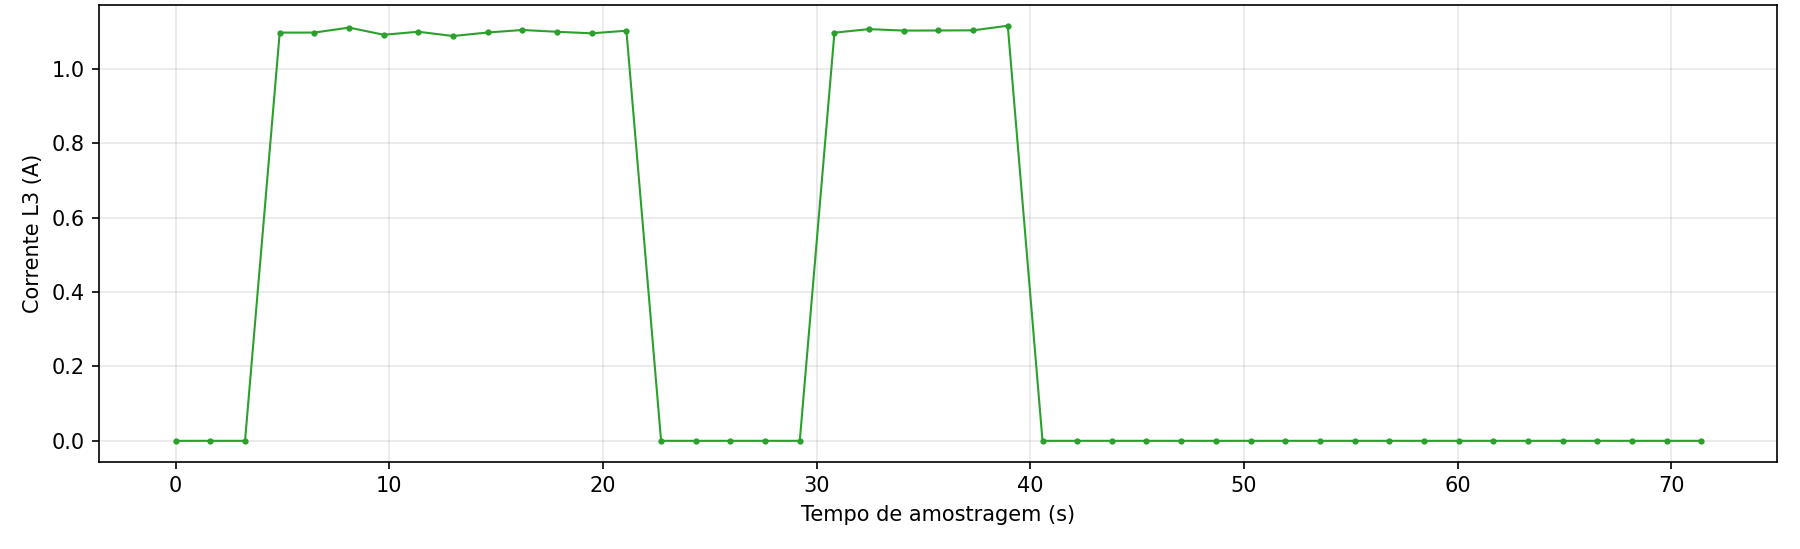
\includegraphics[width=0.85\textwidth]{figuras/I_L3.png}
    \label{fig:corrente_l3}\\
    \autoria{ Autoria Própria.}
\end{figure}

\begin{figure}[htb]
    \centering
    \caption{Tensão de rede registrada durante o ensaio de falta de fase.}
    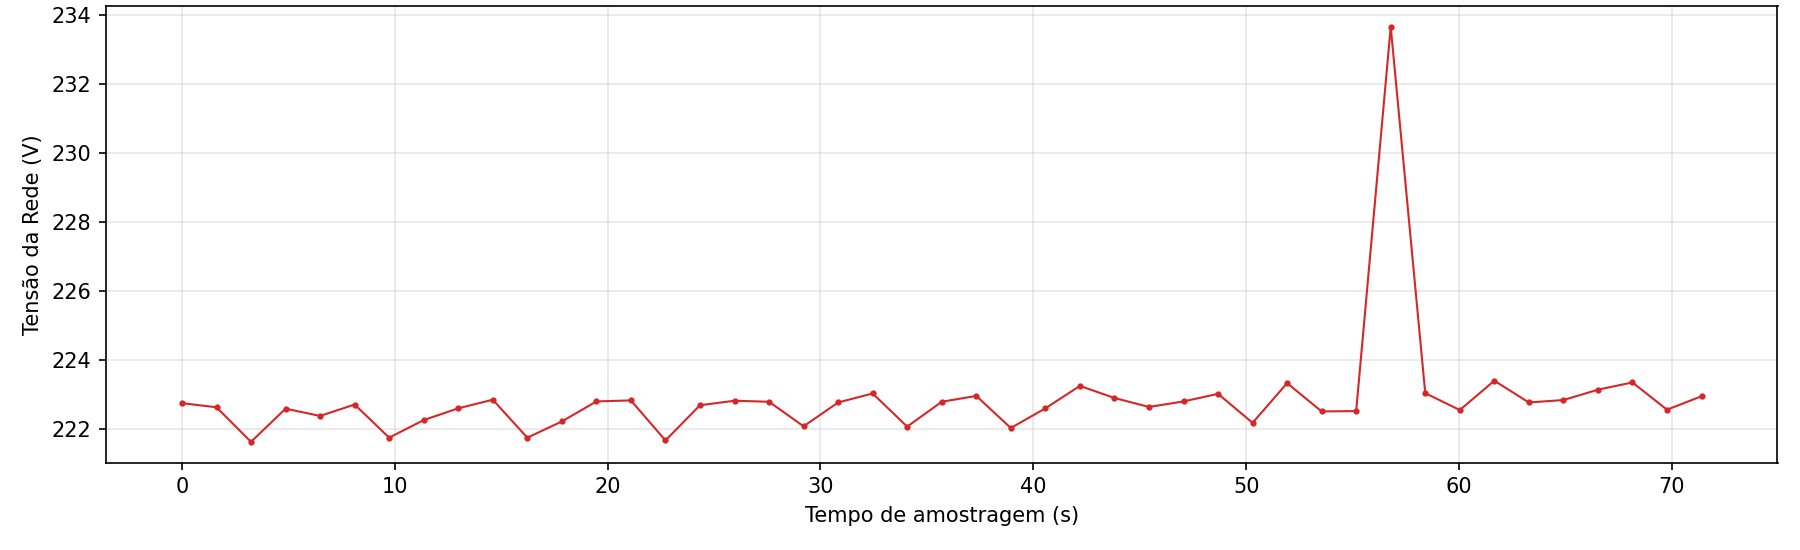
\includegraphics[width=0.85\textwidth]{figuras/V_rede.png}
    \label{fig:tensao_rede}\\
    \autoria{ Autoria Própria.}
\end{figure}

Observa-se, nos primeiros 40 segundos de ensaio, um comportamento
consistente com a operação trifásica equilibrada do motor: as três
fases apresentam corrente próxima de 1,1 A durante os períodos de
regime permanente, com pequenas variações associadas a diferentes
condições de carga impostas pela bancada. A partir de aproximadamente
40 segundos, no entanto, a fase L3 deixa de apresentar corrente,
caracterizando a interrupção proposital dessa fase pela bancada de
testes. Após alguns segundos o sistema é energizado novamente e as fases L1 e L2 registram uma elevação
abrupta de corrente, atingindo valores próximos de 10 A, muito acima da
corrente nominal do motor.


Em relação à tensão de rede Figura~\ref{fig:tensao_rede}, observa-se
que o sistema manteve o valor medido estável, entre 222 V e 223 V,
durante praticamente todo o ensaio, com exceção de uma única amostra
próxima de 57 segundos, na qual foi registrado um valor pontual de
233,6 V.

% De forma geral, os resultados obtidos nos dois ensaios indicam que o
% sistema embarcado foi capaz de registrar corretamente tanto a operação
% em regime permanente quanto a transição para uma condição de falha na
% alimentação elétrica, evidenciando potencial para aplicação em
% cenários de detecção de distúrbios de qualidade de energia, tema que
% será retomado nas considerações finais deste trabalho.